\documentclass{article}
\usepackage{amsmath}
\usepackage{amsfonts}
\usepackage[margin=1in]{geometry}
\usepackage{graphicx}

\DeclareMathOperator{\Pois}{Pois}
\DeclareMathOperator{\Prob}{P}
\DeclareMathOperator{\Exp}{Exp}
\DeclareMathOperator{\Bernoulli}{Bernoulli}
\DeclareMathOperator{\GammaDist}{Gamma}
\DeclareMathOperator{\NegBin}{NegBin}
\DeclareMathOperator{\Erlang3}{Erlang-3}
\DeclareMathOperator{\E}{E}
\DeclareMathOperator{\Var}{Var}
\DeclareMathOperator{\Cov}{Cov}
\DeclareMathOperator*{\argmax}{\arg\!\max}
\def\bs{\boldsymbol}
\def\ibd{\textrm{IBD}}

\def\H{\mathcal{H}}
\def\R{\mathcal{R}}
\def\X{\bs{X}}
\def\m{\mathrm{(m)}}
\def\p{\mathrm{(p)}}
\def\a{\mathrm{(a)}}
\def\b{\mathrm{(b)}}
\def\P{\mathcal{P}}
\def\U{\mathcal{U}}

\begin{document}

\section{Gene conversion}

We are interested in modeling the effects of gene conversion on genome-wide
patterns of genetic variation within clonal asexual lineages. We will begin
with a diploid asexual lineage and then proceed to the more complex case of
triploids. We assume that the asexual lineage is derived from diploid sexual
ancestors.

We work in continuous time, with time scaled by $2N_0$, where $N_0$ is the
(diploid) population size of the sexual ancestor of the asexual lineage. Assume
that this diploid asexual lineage is derived from its sexual ancestors at time
$t=T_d$ in the past, with the present being $t=0$. For the moment we will also
model distances along the genome as continuous variables.

We assume that during the asexual phase of the lineage's ancestry, gene
conversion initiation events occur as a Poisson process in both time and space
(i.e., along the genome).  For the moment, we also assume that each gene
conversion tract is exponentially distributed in length, although we will
return to this assumption later.

In sexually reproducing species, gene conversion can be thought of as a
double-recombination event in the coalescent process. In clonally reproducing
asexual lineages, gene conversion instead acts analogously to coalescence,
since chromosomes are ``trapped'' in the same lineage and each gene conversion
event causes two chromosomes to share ancestry at that point. Since all genetic
differences separating two chromosomes are due to mutations that occurred since
their shared ancestor, we are intersted in the most recent gene conversion time
at each locus: the distribution across the genome of these most-recent gene
conversion times is our object of interest.  See
Fig.~\ref{fig:geneconversiondiagram} for an illustration of the process under
consideration.

\begin{figure}
    \centering
    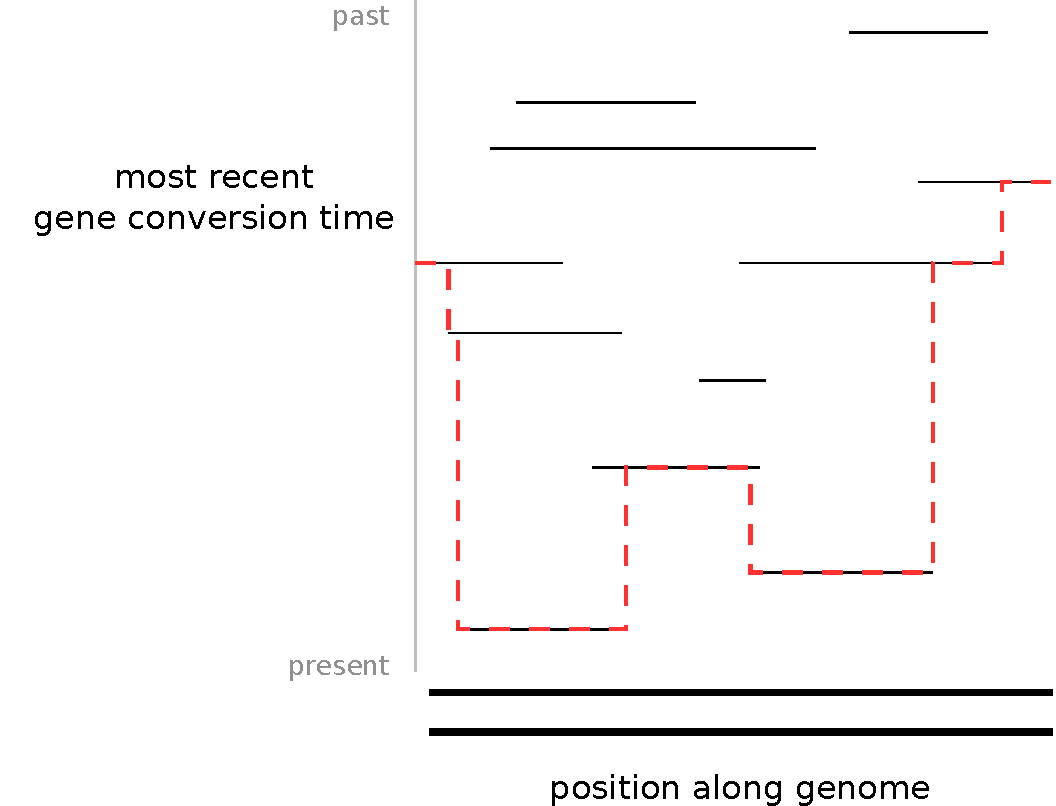
\includegraphics[width=0.7\textwidth]{figs/geneconversion.pdf}
    \caption{
        Schematic of the gene conversion process. Gene conversion events occur
        as a Poisson process in time and along the genome, and each gene
        conversion tract has an exponential length distribution. At each point
        along the two aligned chromosomes, the time of the most recent gene
        conversion event is marked with a dashed red line. We are interested in
        modeling the distribution of this dashed red line across a genome,
        since it determines patterns of genetic variation.}
    \label{fig:geneconversiondiagram}
\end{figure}

With our assumption of a two-dimensional Poisson process, the probability that
a gene conversion event is initiated in the intervals $(x, x+dx)$ along the
genome and $(t,t+dt)$ back in time is $\lambda_c dxdt$ for some rate of gene
conversion $\lambda_c$. The length of a particular gene conversion tract has
the distribution $\lambda_Le^{-\lambda_Lx}$ so that the mean gene conversion
tract length is $1/\lambda_L$.

Going back in time at a particular locus, the probability that that particular
locus is affected by a gene conversion event in the time interval $(t, t+dt)$
is 

\begin{align*}
    &= \lambda_c dt \int_0^{\infty} dx \Prob(L>x)\\
    &= \lambda_c dt \E[L]\\
    &= \frac{\lambda_c}{\lambda_L}dt,
\end{align*}
where $L$ is the random length of a gene conversion tract. In the second
equality we use the fact that $\int_0^\infty \Prob(L>x)dx = \E[L]$ for any
non-negative random variable $L$. (Thus, this holds for all gene conversion
tract length distributions.) In other words, the rate of
encountering a gene conversion tract that causes shared ancestry between the
two chromosomes at a particular location in the genome is the rate of
initiation of these events in time multiplied by the mean length of a tract.

Under the assumption of an exponential tract length distribution, the end of
the current tract is encountered with rate $\lambda_Ldx$. It is also possible
that we encounter a more recent gene conversion event that causes a more recent
common ancestor event between the two chromosomes. Given the current gene
conversion time $s$, this happens at rate $\lambda_c s dx$. Thus the total rate of
encountering the a change in gene conversion time is
$(\lambda_L+\lambda_cs)dx$.

Given that a more recent gene conversion time is encountered, the age of this
gene conversion time is uniformly distributed in $[0,s)$. Given that the end of
the tract is encountered, the next gene conversion event is encountered (going
back in time from $s$) at rate $\lambda_c/\lambda_L dt$, as before.
\textbf{Crucially, this assumes that gene conversion events do not overlap.} In
reality, gene conversion events will overlap, and the full process cannot be
described by a Markov jump process. We will make the assumption that gene
conversion tracts do not overlap completely (example shown in
Fig.~\ref{fig:overlap}), and thus our model can be described by a first-order
Markov chain. It is possible to make the model a second-order Markov chain and
allow pairwise overlap, as in Yin et al.\ 2009 (\textit{Bioinformatics},
25:231-239), but this nearly squares the number of states to consider, so the
viability of this will have to be considered later.

\begin{figure}
    \centering
    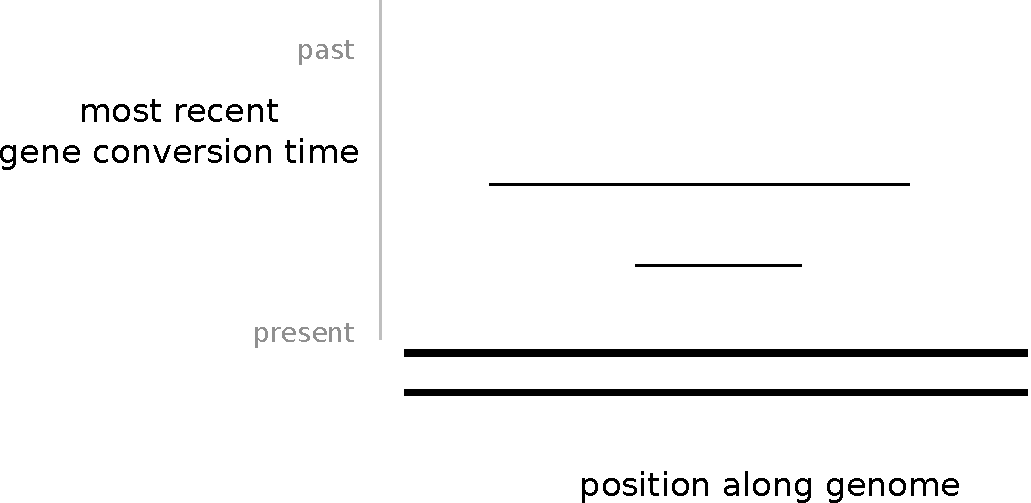
\includegraphics[width=0.5\textwidth]{figs/overlap.pdf}
    \caption{Example of full overlap in gene conversion tracts. Because of
    events like this, the gene-conversion process cannot be described by a
    first-order Markov model. In our model we assume that events such as this
    cannot occur, enabling a description by a first-order Markov process.}
    \label{fig:overlap}
\end{figure}

Considering the above, the local gene conversion time changes along the genome
at rate $(\lambda_L + s\lambda_c)dx$, and at a transition site, the density of
next gene conversion time is

\begin{equation}
    r(t|s)dt = 
    \begin{cases}
        \frac{\lambda_c}{s\lambda_c+\lambda_L}dt & 0<t<s\\
        \frac{\lambda_c}{s\lambda_c+\lambda_L}e^{-\frac{\lambda_c(t-s)}{\lambda_L}}dt &  t>s.\\
    \end{cases}
\end{equation}


\end{document}
